% p41-a-typical-element-of-the-basis-u0.tex
%
% Source: Carl A. Gunter and Dana S. Scott, "Semantic Domains".
%   physical page 41 of ScottDomains/papers/Gunter Scott 1990.pdf
%   printed page 40
%   section 7.3, "Solving domain equations with projections."
%   unnamed in the paper; introduced by this sentence:
%
%   "We begin by describing the basis of a domain U.  Let S be the set of
%    rational numbers of the form n/2^m where 0 <= n < 2^m and 0 < m.  As the
%    basis U_0 of our domain we take finite (non-empty) unions of half open
%    intervals [r,t) = {s in S | r <= s < t}.  A typical element would look
%    like"
%
% What it shows: one element of U_0 — a finite union of half-open intervals of
% dyadic rationals, drawn as the thick stretches of the ambient interval, each
% boundary marked ")[" because the intervals are closed on the left and open on
% the right.  The next page orders these sets by superset, so [0,1) is the
% least element, and shows the resulting Boolean algebra is countable and
% atomless — which is what makes U universal (Theorem 27).
%
% *** This diagram is a false negative of scripts/find-diagrams.py. ***  It is
% not in analyses/diagram-candidates.2026-0808-10:32.orchestrator.log at all:
% the detector separates rows by ink density, and this picture is one glyph row
% tall, so it never reached the height threshold.  Page 41's two candidate rows
% are the F_1..F_n display and the p-representability square, not this.
%
% Geometry: measured exactly, from the page content stream.  `mutool draw -F
% trace` on physical page 41 reports the picture as 14 glyphs on the single
% baseline y = 97.43: seven "[" (font glyph 104) at x = 159.60, 195.60, 231.60,
% 303.60, 339.60, 375.60, 411.60 and seven ")" (glyph 17) at x = 193.92,
% 229.92, 301.92, 337.92, 373.92, 409.92, 445.92.  So the ambient interval runs
% 159.6 to 447.6 pt = 288 pt, divided into eight cells of 36 pt, and the six
% internal boundaries fall at cells 1, 2, 4, 5, 6, 7.  One cm here is 36 pt
% there.  Which cells are inked thick was read off 600 dpi crops of the two
% halves: cells 2, 5 and 7 of 8, that is [1/8,1/4) u [1/2,5/8) u [3/4,7/8).
% Note the gap between the first and second interval is two cells wide, which
% is why the trace has no glyph pair at the 267.6 pt grid line — the paper
% marks only the boundaries of the intervals it draws.

\documentclass[border=6pt]{standalone}
\usepackage{tikz}
\begin{document}
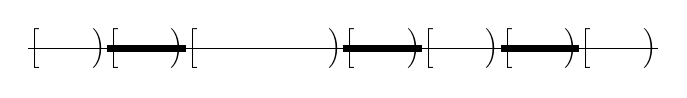
\begin{tikzpicture}[
  x=1cm, y=1cm,
  every node/.style={inner sep=1pt},
  open/.style={circle, draw, fill=white, minimum size=4pt, inner sep=0pt},
  solid/.style={circle, draw, fill=black, minimum size=5pt, inner sep=0pt},
  edge/.style={draw, line width=0.4pt},
  obj/.style={inner sep=3pt},
  arrow/.style={draw, line width=0.4pt, ->},
  darrow/.style={draw, line width=0.4pt, ->, dash pattern=on 4pt off 3pt},
  % scale=0.8: in the paper a bracket is 17.3 pt tall against a 36 pt cell, a
  % ratio of 0.48; an unscaled \Big here measures 70 px against a 118 px cell
  % at 300 dpi, a ratio of 0.59.  0.8 brings it to the paper's proportion.
  bracket/.style={inner sep=0.5pt, scale=0.8},
  thickpart/.style={draw, line width=2.4pt}]

  % ---- the ambient interval, drawn thin the whole way ---------------------
  \draw[edge] (0,0) -- (8,0);

  % ---- the three half-open intervals of this element, drawn thick ---------
  \draw[thickpart] (1,0) -- (2,0);
  \draw[thickpart] (4,0) -- (5,0);
  \draw[thickpart] (6,0) -- (7,0);

  % ---- the ends of the ambient interval -----------------------------------
  \node[bracket, anchor=west] at (0,0) {$\Big[$};
  \node[bracket, anchor=east] at (8,0) {$\Big)$};

  % ---- the six internal boundaries, each printed as ")[" ------------------
  \node[bracket, anchor=east] at (1,0) {$\Big)$};
  \node[bracket, anchor=west] at (1,0) {$\Big[$};
  \node[bracket, anchor=east] at (2,0) {$\Big)$};
  \node[bracket, anchor=west] at (2,0) {$\Big[$};
  \node[bracket, anchor=east] at (4,0) {$\Big)$};
  \node[bracket, anchor=west] at (4,0) {$\Big[$};
  \node[bracket, anchor=east] at (5,0) {$\Big)$};
  \node[bracket, anchor=west] at (5,0) {$\Big[$};
  \node[bracket, anchor=east] at (6,0) {$\Big)$};
  \node[bracket, anchor=west] at (6,0) {$\Big[$};
  \node[bracket, anchor=east] at (7,0) {$\Big)$};
  \node[bracket, anchor=west] at (7,0) {$\Big[$};
\end{tikzpicture}
\end{document}
